\chapter{Git (II) - Collaborating With Others}
\label{sec:git2}
% Old Ch. 8

\textit{Advanced Chapter}
\vspace{6mm}

The commands introduced in \cref{sec:ch3} is only enough for working alone, mainly the normal \texttt{git add .; git commit -m "message"; git push} procedure. Things are slightly more hectic when you have more than one person working together in the same repository concurrently. 

\section{The ideal situation}

To make things simple, only one user should work on the project at a time. After someone has finished working, they push their code to GitHub. Then all other people would get the latest code from GitHub and download it to their local device using \texttt{git pull} before they start working on their part of the code. 

\begin{figure}[h]
\centering
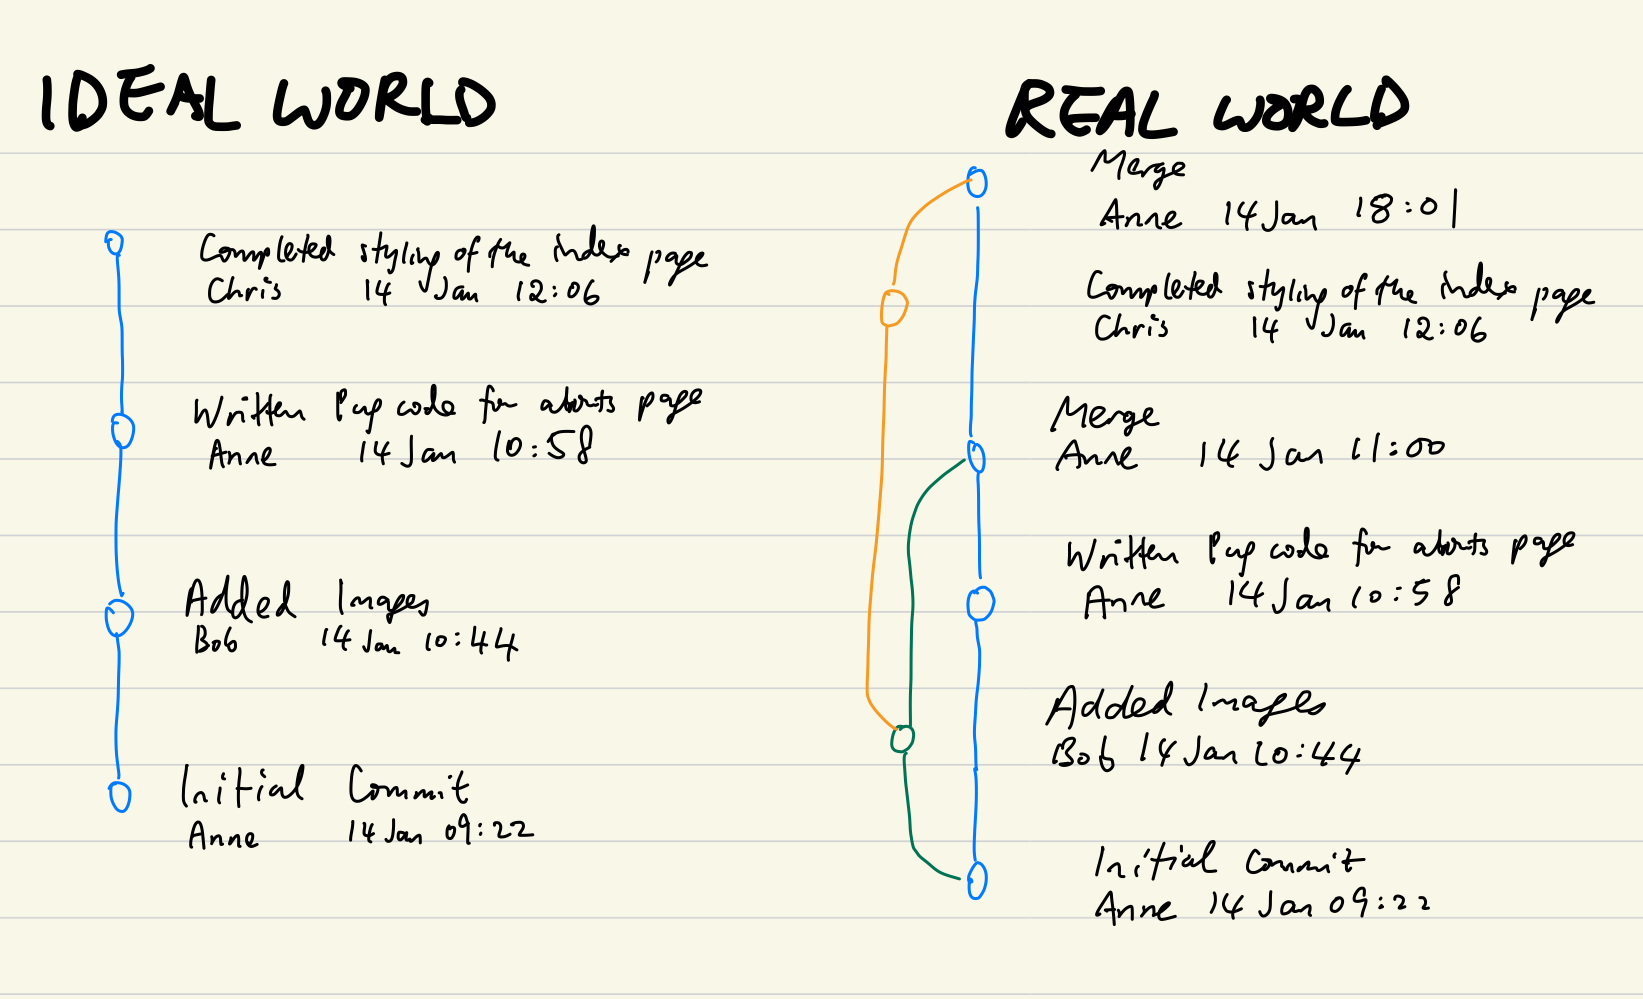
\includegraphics[width=15cm]{images/ch8-messy-git-world.png}
\caption{Messy world of Git}
\end{figure}

Of course, the above method is inefficient, our greediness demands multiple people to be able to work on the code at the same time. Or sometimes people simply forgot to \textbf{pull} (fancier word for download) the latest version of the code before they start working. We have to accept the fact that our \textbf{commit history} (fancier term for edit history) is not a straight line and diversions are unavoidable, just like our lives.\footnote{For fun: life is not a straight line \url{https://amandalinehan.com/life-is-not-a-straight-line/}} We will discuss git commands and techniques that can help you to work with different people in this chapter.

\section{Know what others are doing}
\label{sec:gitpull}

Git operates offline on its own on your local machine unless you request it to look at the changes on GitHub.

As indicated in the previous section, we use \texttt{git pull} to download the updates of the code from GitHub (the cloud) to our local machine. Pull is another word for download.

Note the distinction between \texttt{git pull} and \texttt{git clone} (see \cref{sec:gitclone}). \texttt{git clone} is to copy the repository to your local device, it is only used to download the code initially. \texttt{git pull} is used for subsequent downloads, which aims to update the local code with newest changes.

But sometimes, you just want to see what's made by others before pulling the code. You can do so by \texttt{git fetch}. It updates the local machine what's going on in the GitHub repository, but will not download any code, you can view the updates using one of the visualisation tools in \cref{sec:sublime}.

Visualisation tools are super useful throughout this chapter as they let you see what's going on on different branches in a fashion that is similar to my illustrations.

\begin{figure}[h]
\centering
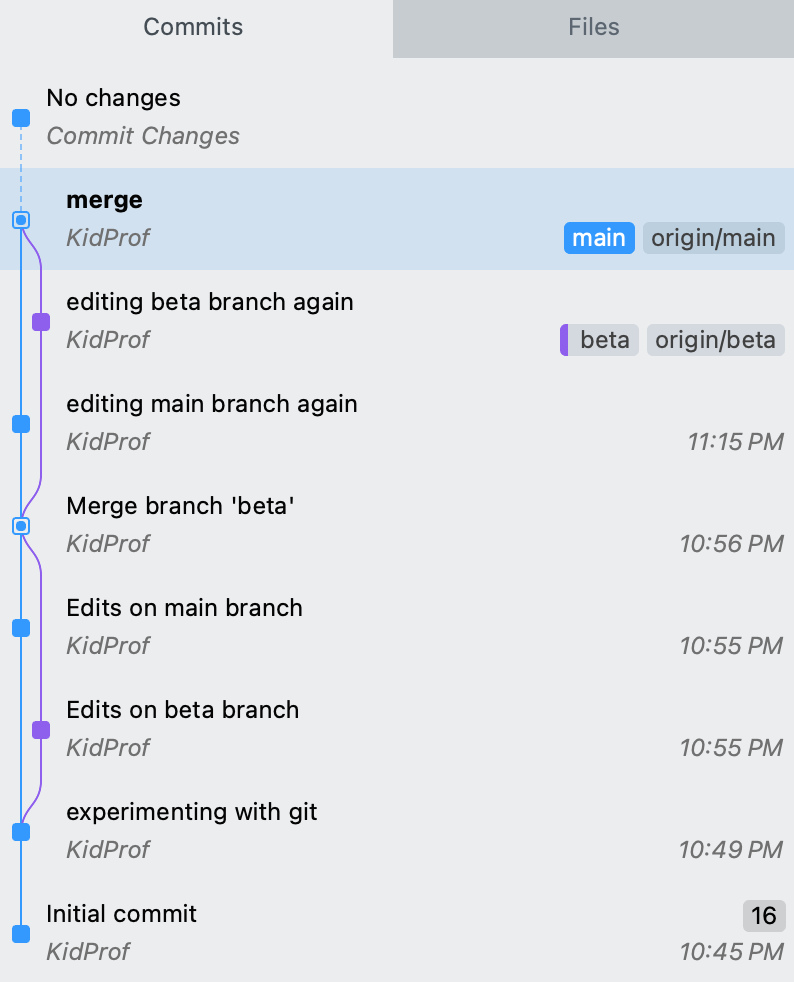
\includegraphics[width=7cm]{images/ch8-sublimemerge.png}
\caption{What sublime merge shows following the tutorial up to \cref{sec:mergeconflict}}
\end{figure}

\section{Branching out}
\label{sec:branch}

We use branches to maintain different versions of the same project. 

\subsection*{Switching between branches}

Creating a new branch using \texttt{git checkout -b} followed by the branch name you want. In the example below, we switched from main branch to our newly created beta branch. The newly created branch has the same contents as the branch you switched from.

To switch to an existing branch, we use \texttt{git checkout}. Note that for subsequent switches to the beta branch you don't need \texttt{-b} anymore, since the beta branch was created already it is now an existing branch.

\begin{lstlisting}[language=bash]
# KidProf in ~/code/git-tutorial on git:main x [22:38:58]
$ git checkout -b beta
Switched to a new branch 'beta'

# KidProf in ~/code/git-tutorial on git:beta x [22:39:12]
$ git checkout main
Switched to branch 'main'

# KidProf in ~/code/git-tutorial on git:main x [22:40:58]
$ git checkout beta
(Note no need -b here because beta is now an existing branch)
Switched to branch 'beta'

# KidProf in ~/code/git-tutorial on git:beta x [22:44:10]
\end{lstlisting}

In Git Bash and MacOS zsh (see \cref{sec:iterm} for set up) you can see the branch that you are currently in.

\subsection*{Making edits}

Switching between branches is now not particularly interesting, so let's now change that.

In the beta branch, we can try opening a random file and change its contents. Ideally mention something about the beta branch for easier recognition.

\begin{lstlisting}[language=pug]
//- app/templates/views/index.pug
extends ../layouts/default

block content
	.container
		h1 Welcome to Static Web!
		br
		p A very cool website.
		p This web is made for tutorial purposes.
		p Edits on beta branch in index page.
\end{lstlisting}

Commit your changes, using the three steps mentioned in \cref{sec:gcmsg}

\begin{lstlisting}[language=bash]
$ git add .
$ git commit -m "edits on beta branch"
$ git push
\end{lstlisting}

You might need to run \texttt{git push --set-upstream origin beta} instead because this is the first push of a new branch. 

Then let's switch back to main branch using \texttt{git checkout main}. Open the file you have modified in the beta branch, you will realise your edits are gone!

This is because we are now at the main branch, and you were making edits on the beta branch instead. Changes on one branch will not affect other branches, this is how you are able to maintain different versions of the same project.

We can make further experimentation with branches by making edits in the main branch also. I deliberately made edits to a different file, the reason will become apparent in the next section.

\begin{lstlisting}[language=pug]
//- app/templates/views/abouts.pug
extends ../layouts/default

block content
	.container
		p abouts page
		p Edits on main branch in abouts page.
\end{lstlisting}

\begin{lstlisting}[language=bash]
$ git add .
$ git commit -m "edits on main branch"
$ git push
\end{lstlisting}

Now you can switch back and forth between the two branches and see that the contents are different.

\begin{figure}[h]
\centering
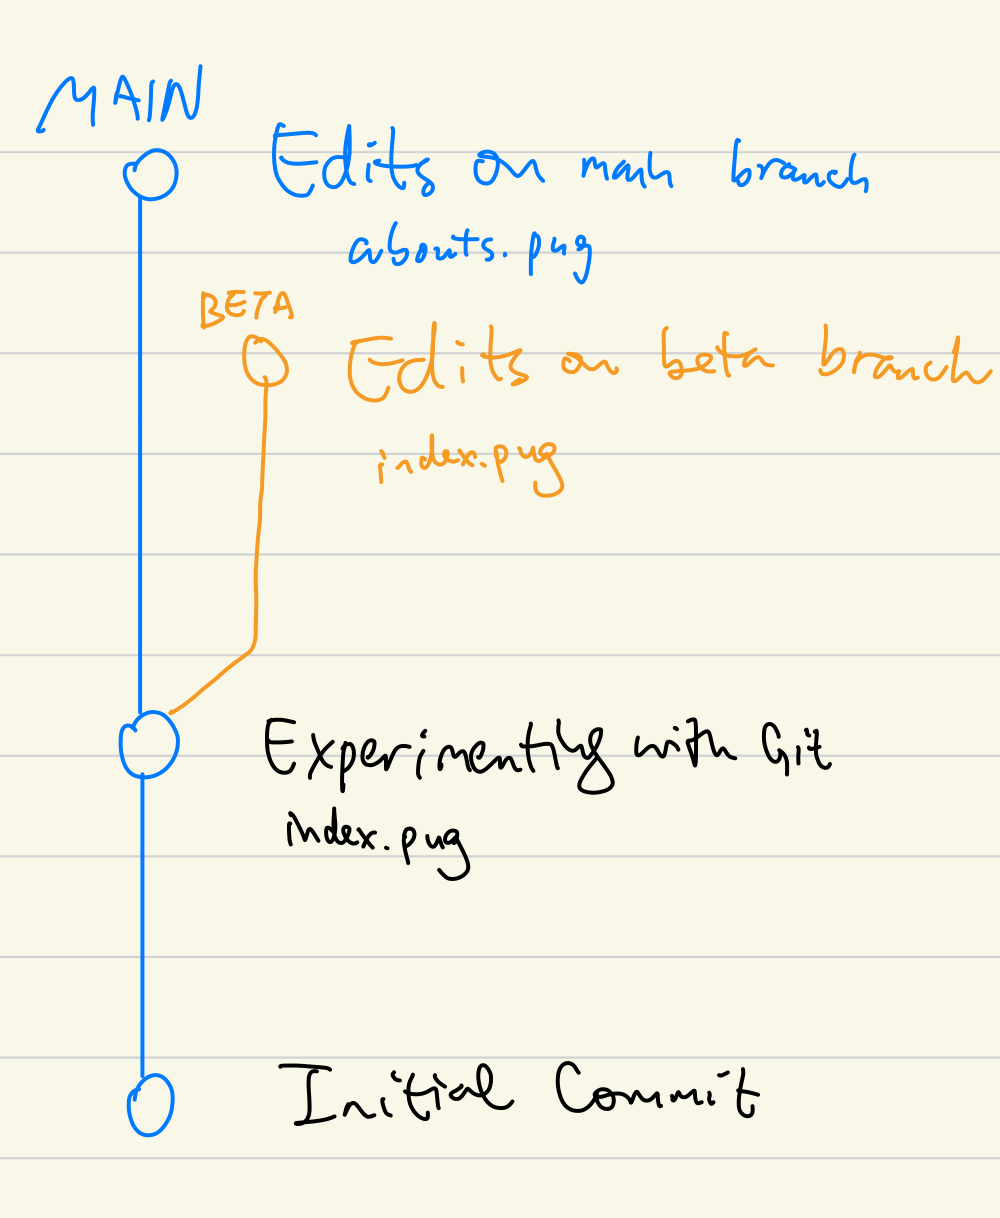
\includegraphics[width=7cm]{images/ch8-branching.png}
\caption{Visualising the two branches created}
\end{figure}

\subsection*{Uses of branches}
Yes we use branches to maintain different versions of the same project. The common practice will be each employee of a company work on their own branch named after their name (e.g. dev-kidprof), so that they can work on their own tasks without interfering with others.

However, we only want one version at the end, the version that you publish to the public. To achieve this, the employees will \textbf{merge} their branches (see next section) back to the main branch. The main branch usually is the final product of the project and it should be relatively error free because all known issues should be resolved before merging code from other branches to the main branch.

\section{Merging}
\label{sec:merge}

\subsection{Merge Without Conflicts}

We will try to merge the beta branch into the main branch (i.e. apply the changes in beta branch to the main branch)

We can do so by first checking out to the main branch, the branch that you want to merge into.
\vspace{6mm}

\begin{lstlisting}[language=bash]
$ git checkout main
\end{lstlisting}

\vspace{6mm}
Then run the command \texttt{git merge}, to merge the beta branch into the main branch.

\vspace{6mm}\begin{lstlisting}[language=bash]
$ git merge beta
\end{lstlisting}
\vspace{6mm}

A command line text editor may pop up, we do not need to modify anything. So we can just type \texttt{:wq} then tap enter to quit the text editor and save. For more information on how to control the command line text editor, refer to \cref{sec:vim}.

When you check your code, your edits in both the index page and abouts page are there. :)

Finally, push our merge to GitHub with \texttt{git push}.
\vspace{6mm}

If you want your beta branch to obtain the updates from the main branch, we can do the same for beta branch, that is:
\vspace{6mm}

\begin{lstlisting}[language=bash]
$ git checkout beta
$ git merge main
$ git push
\end{lstlisting}

\begin{figure}[h]
\centering
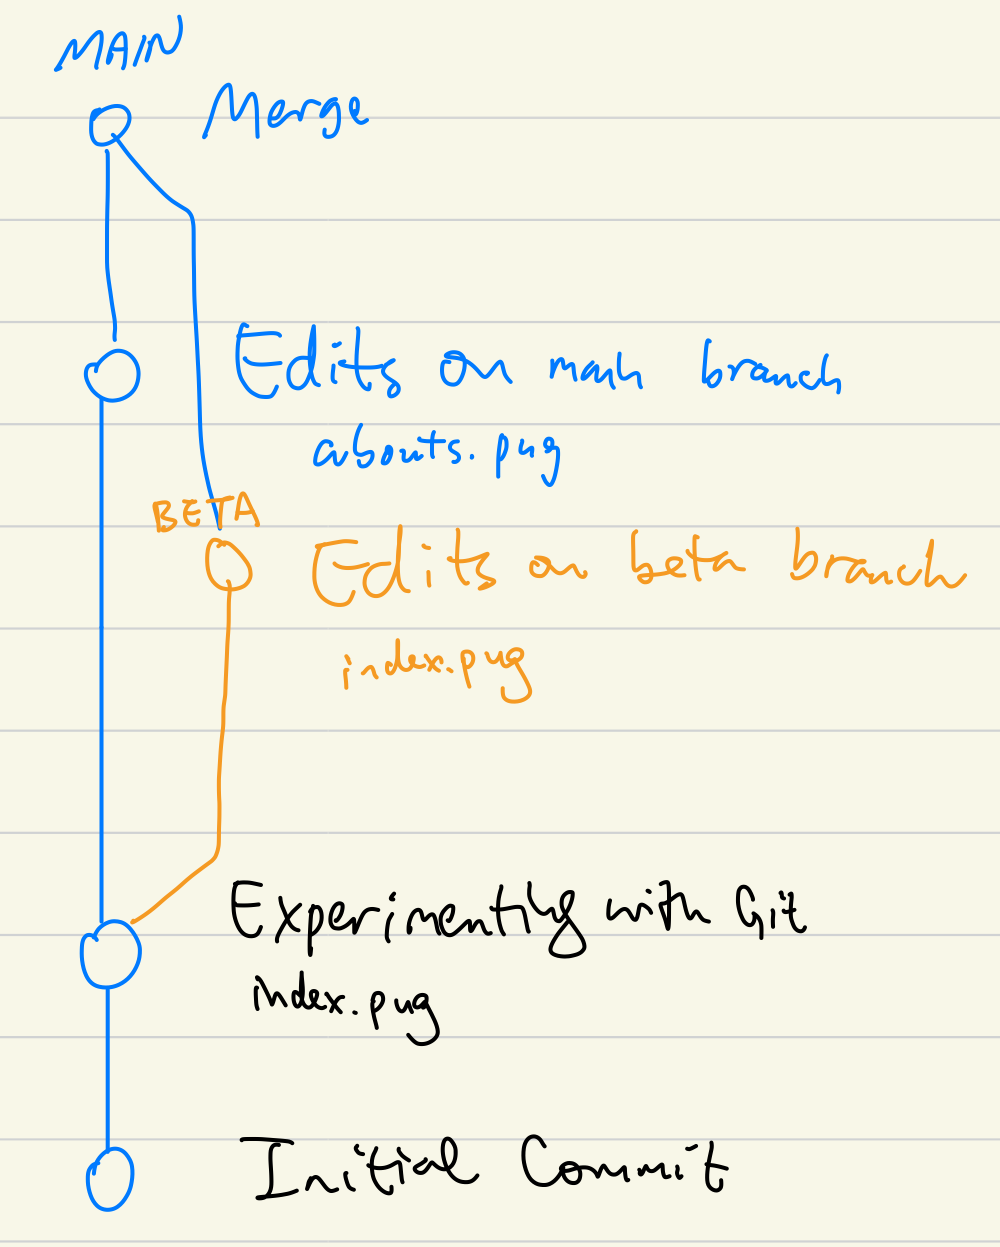
\includegraphics[width=7cm]{images/ch8-merge-safe.png}
\caption{Visualising the merge}
\end{figure}

\subsection{Merge Conflict}
\label{sec:mergeconflict}
The merge just now seems a bit too easy, that is because the two branches edited different files. The merging process would be more interesting when both branches edit the same part of the file. The following illustrates an example.
\vspace{6mm}

We first go to main branch and add a new line in \texttt{index.pug}.
\vspace{6mm}

\begin{lstlisting}[language=bash]
$ git checkout main
\end{lstlisting}

\begin{lstlisting}[language=pug]
//- app/templates/views/index.pug
...
p This web is made for tutorial purposes.
p Edits on beta branch in index page.
p New line on main branch.
\end{lstlisting}

\begin{lstlisting}[language=bash]
$ git add .
$ git commit -m "editing main branch again"
git push
\end{lstlisting}
\vspace{6mm}

Then we go to the beta branch and do the same. You will see the edits you have made just now and also the edits you have made for abouts page are missing, that is because we are in a different branch.
\vspace{6mm}

\begin{lstlisting}[language=bash]
$ git checkout beta
\end{lstlisting}

\begin{lstlisting}[language=pug]
//- app/templates/views/index.pug
...
p This web is made for tutorial purposes.
p Edits on beta branch in index page.
p New line on beta branch.
\end{lstlisting}

\begin{lstlisting}[language=bash]
$ git add .
$ git commit -m "editing beta branch again"
$ git push
\end{lstlisting}
\vspace{6mm}

Then we go back to main branch and try to merge beta branch into main branch.
\vspace{6mm}

\begin{lstlisting}[language=bash]
$ git checkout main

# KidProf in ~/code/git-tutorial on git:main o [23:28:42]
$ git merge beta
Auto-merging app/templates/views/index.pug
CONFLICT (content): Merge conflict in app/templates/views/index.pug
Automatic merge failed; fix conflicts and then commit the result.
\end{lstlisting}
\vspace{6mm}

When you run \texttt{git status}, you can see it tells you that both branches modified \texttt{index.pug}.
\vspace{6mm}

\begin{lstlisting}[language=bash]
$ git status
On branch main
Your branch is up to date with 'origin/main'.

You have unmerged paths.
  (fix conflicts and run "git commit")
  (use "git merge --abort" to abort the merge)

Unmerged paths:
  (use "git add <file>..." to mark resolution)
	both modified:   app/templates/views/index.pug
\end{lstlisting}
\vspace{6mm}

When you open VS code, you may see the conflicting part of the code.
\vspace{6mm}

\begin{figure}[h]
\centering
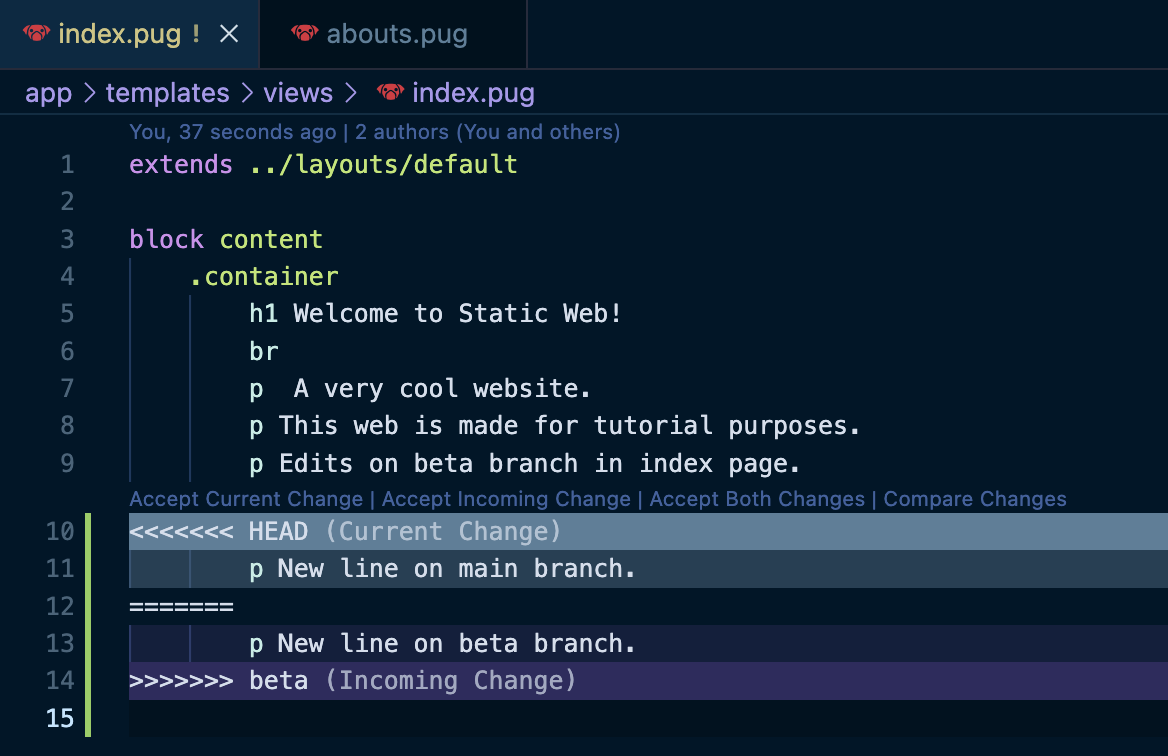
\includegraphics[width=12cm]{images/ch8-merge-conflict-vscode.png}
\caption{Visualising the merge}
\end{figure}

But let's do it in the hardcore way, you don't need any more additional tools to fix a merge other than a plain text editor. 

\begin{lstlisting}[language=pug]
extends ../layouts/default

block content
	.container
		h1 Welcome to Static Web!
		br
		p  A very cool website.
		p This web is made for tutorial purposes.
		p Edits on beta branch in index page.
<<<<<<< HEAD
		p New line on main branch.
=======
		p New line on beta branch.
>>>>>>> beta
\end{lstlisting}
\vspace{6mm}

As you can see, it uses arrows to indicate the area of the conflict, and listed both versions separately with = symbols in the middle. What you should do is merge the changes of the two versions and remove the arrows and = symbols, and Git will regard that conflict as fixed. 

In this example, let's change it to \texttt{New line on both branches.} Remove all the arrow and = symbols.

You can learn more how to merge in general with a bit more practice and below in one of the FAQs before \hyperref[sec:mergefaq]{the end of this subsection.}
\vspace{6mm}

\begin{lstlisting}[language=pug]
//- app/templates/views/index.pug
extends ../layouts/default

block content
	.container
		h1 Welcome to Static Web!
		br
		p  A very cool website.
		p This web is made for tutorial purposes.
		p Edits on beta branch in index page.
		p New line on both branches.
\end{lstlisting}
\vspace{6mm}

Finally, we just use the daily routine to push our merged code to GitHub. If no errors appear when running \texttt{git add .}, it means you have merged the code successfully.
\vspace{6mm}

\begin{lstlisting}[language=bash]
$ git add .
$ git commit -m "merge"
$ git push
\end{lstlisting}

\subsection*{When would there be a conflict when merging?}

When both branches modify the same part of the same file. (If two branches modify different parts of the file, there might not be one if Git recognises that the two edits are far away enough.)

\subsection*{Which changes should I choose when there is a conflict?}
\label{sec:mergefaq}
It heavily depends on the situation! The Git tools provided by VS code may make you think only changes from one of the branch can be taken and we must discard the other, this is definitely not the case. The product of the merge should be what you want to be in your project finally. Maybe one of them is more updated, maybe you need to incorporate elements on both changes. For example, one branch may changed the indentation of a part of the code because they are now put in an if clause, while the other branch edited the contents of one line of the code. What you actually want is neither of them, but you need both the indentation change and content change. There is another slightly more elaborate example in the next section.

\subsection*{Is merge conflict bad?}

Not at all, different versions of code would definitely appear as multiple people edit the code in parallel. \texttt{git merge} provides you with a systematic tool to merge the differences and create one single final product. (It is much more better than working with different zip files right?) As long as you don't panic and merges the code correctly, aiming at making the final product better and bug free, it is completely fine. 

\section{Merges due to edits on the same branch}
\label{sec:mergesamebranch}

It is not a must for different people to make edits on their own branch, multiple people could be working on the same branch for convenience. But there must only be one most updated version of the branch at a given time, so Git will refuse to push your code when somebody else has made edits on the same branch previously that you haven't pulled. 

This is best done using two people, the two people will be Anne and Bob in my example. \footnote{You can sort of simulate that by having two copies of the same project on your device by leaving the current project directory and then running \texttt{git clone $<$url$>$ git-tutorial-2}. (but this is not ideal as you may just get yourself confused.)}

This is very similar to the last section, we are also merging two different versions of code, but this time they are from the same branch, that means we must merge it as there must only be one version of the branch at a given time. However, in the previous section, we can delay our merge to whenever we need to.

First, Anne made some edits in the abouts page in the main branch. 
\vspace{6mm}

\begin{lstlisting}[language=bash]
# Anne
$ git checkout main
\end{lstlisting}

\begin{lstlisting}[language=pug]
//- Anne: app/templates/views/abouts.pug
extends ../layouts/default

block content
	.container
		p abouts page
		p Edits on main branch in abouts page.

		h1 Self introduction
		ul
			li Anne: Hi I am Anne I love coding.
\end{lstlisting}

\begin{lstlisting}[language=bash]
# Anne
$ git add .
$ git commit -m "added self intro section and Anne's description"
$ git push
\end{lstlisting}
\vspace{6mm}

Then Bob made similar changes, probably he isn't told that Anne has worked on it already.
\vspace{6mm}

\begin{lstlisting}[language=bash]
# Bob
$ git checkout main
\end{lstlisting}

\begin{lstlisting}[language=pug]
//- Bob: app/templates/views/abouts.pug
extends ../layouts/default

block content
	.container
		p abouts page
		p Edits on main branch in abouts page.

		h2 Self introduction
		ul
			li Bob: Hi I am Bob I love programming.
\end{lstlisting}

As Anne made some changes earlier, Bob cannot push his code as smoothly.

\begin{lstlisting}[language=bash]
# Bob
$ git add .
$ git commit -m "added self intro section and Bob's description"
$ git push
To github.com:KidProf/git-tutorial.git
 ! [rejected]        main -> main (fetch first)
error: failed to push some refs to 'github.com:KidProf/git-tutorial.git'
hint: Updates were rejected because the remote contains work that you do
hint: not have locally. This is usually caused by another repository pushing
hint: to the same ref. You may want to first integrate the remote changes
hint: (e.g., 'git pull ...') before pushing again.
hint: See the 'Note about fast-forwards' in 'git push --help' for detail
\end{lstlisting}

Git advises Bob to first pull the code from the main branch. After running \texttt{git pull}, the situation would be the \textbf{same as the previous section}. What need to do depends on whether there are merge conflicts. If there are no merge conflicts, you just need to add commit and push your merge.

We were told by Git that unfortunately there is a merge conflict at \texttt{abouts.pug}, as you should expect as both Anne and Bob modified the same part of the abouts page.

\begin{lstlisting}[language=pug]
//- Bob: app/templates/views/abouts.pug
extends ../layouts/default

block content
	.container
		p abouts page
		p Edits on main branch in abouts page.
<<<<<<< HEAD
		h2 Self introduction
		ul
			li Bob: Hi I am Bob I love programming.
=======
		h1 Self introduction
		ul
			li Anne: Hi I am Anne I love coding.
>>>>>>> 484fb78c7ac9f62c53cd8b87529e91d5252a60e9
\end{lstlisting}

We definitely want both of their self introductions in the final product, and we can choose between \texttt{h1} and \texttt{h2} and see which one is more aesthetically pleasing. Let's choose \texttt{h2} for now. Make sure to remove the arrows and = signs after you are finished. 
\vspace{6mm}

\begin{lstlisting}[language=pug]
//- Bob: app/templates/views/abouts.pug
extends ../layouts/default

block content
	.container
		p abouts page
		p Edits on main branch in abouts page.
		h2 Self introduction
		ul
			li Bob: Hi I am Bob I love programming.
			li Anne: Hi I am Anne I love coding.
\end{lstlisting}
\vspace{6mm}

Then we just continue with the normal procedure. This is what you should do as well when there are no merge conflicts.
\vspace{6mm}

\begin{lstlisting}[language=bash]
# Bob
$ git add .
$ git commit -m "merge"
$ git push
\end{lstlisting}

\begin{figure}[h]
\centering
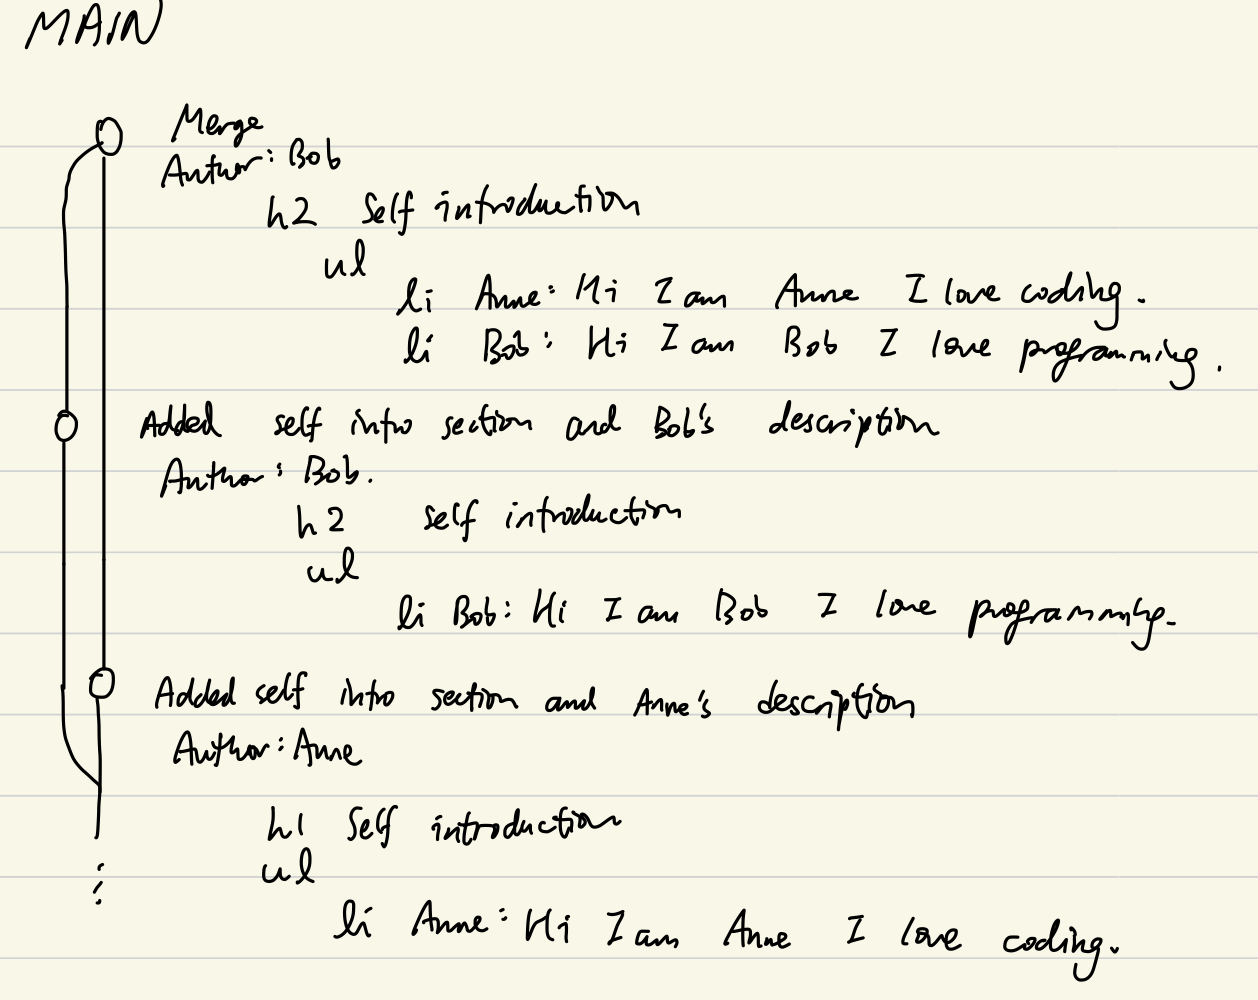
\includegraphics[width=15cm]{images/chn5-same-branch-merge.png}
\caption{Visualising the merge}
\end{figure}

% \section{Stashing}

% \textit{Of less importance}
% \vspace{6mm}

% A temporary local area for you to store your edits. When you think your local edits are useful/ not ready to push but you need to work on other branches immediately. You can temporarily store your code on your local machine using \texttt{git stash}. More information on how to use is in the git commands table below.

\section{Something went wrong?}

Branching, merging and merge conflicts are unavoidable when working with different people using Git. They might be intimidating at first (especially merge conflict), you can refer to tips in \cref{sec:gitpractice} if anything goes wrong. Practice makes perfect is always the way to go for Git. 

To add to the list, another thing you can do if you find it difficult to solve the merge conflict, run \texttt{git merge --abort} to stop the merge, then create a new temporary branch, and push your code there first. Then merge when you feel more comfortable or under supervision of a more experienced Git developer.

\begin{table}[H]
    \centering
    \caption{Table of common Git commands}
    \vspace{6mm}
    \begin{tabular}{|m{7em}|m{23em}|}
        \hline
        \textbf{Command} & 
        Description 
        \\ \hline \hline
        
        \texttt{git add .} &
        First step to push your code to GitHub - includes all the changes in the folder to be ready for a commit (\cref{sec:gcmsg})
        \\ \hline
        
        \texttt{git commit -m "message"} &
        Second step to push your code to GitHub - seals and confirms your changes into one chunk, and adds a commit message (\cref{sec:gcmsg})
        \\ \hline
        
        \texttt{git push} &
        Third step to push your code to GitHub - uploads the commit from your local machine to GitHub (\cref{sec:gcmsg})
        \\ \hline
        
        \texttt{git init} &
        Initialises a new Git repository in the current folder on your local machine (\cref{sec:gitinit})
        \\ \hline
        
        \texttt{git clone $<$url$>$} &
        Creates a new folder with the repository name would be created with all the code inside (\cref{sec:gitclone})
        \\ \hline
        
        \texttt{git pull} &
        Downloads the updates of the code from GitHub to our local machine (\cref{sec:gitpull})
        \\ \hline
        
        \texttt{git fetch} &
        Updates the local machine what's going on in the GitHub repository, but will not download any code. (\cref{sec:gitpull})
        \\ \hline
        
        \texttt{git checkout -b $<$branch$>$} &
        Creates a new branch (\cref{sec:branch})
        \\ \hline
        
        \texttt{git checkout $<$branch$>$} &
        Moves to another existing branch (\cref{sec:branch})
        \\ \hline
        
        \texttt{git merge $<$branch$>$} &
        Merges the updates on the specified branch into the current branch. (\cref{sec:merge})
        \\ \hline
        
        % \texttt{git stash -u} &
        % Save current changes, including new (untracked) files (\cref{sec:gitstash})
        % \\ \hline
        
        % \texttt{git stash pop} &
        % Apply the changes you recently saved. (\cref{sec:gitstash})
        % \\ \hline
        
        % \texttt{git stash clear} &
        % Remove all stashes. (\cref{sec:gitstash})
        % \\ \hline
        
    \end{tabular}
\end{table}
